\documentclass{scu-thesis}
% \usepackage{graphicx}	% for including graphics
% \usepackage{amsmath}	% for advanced typesetting of mathematics
% \usepackage{txfonts}	% for using the Times-Roman font
% \usepackage{natbib}	% for better citation styles
\usepackage[utf8]{inputenc}
\usepackage{amstext}
\usepackage{setspace}
\usepackage{pdflscape}
\usepackage{color}
\usepackage[table]{xcolor}
\usepackage{amsmath}
\usepackage{graphicx}
\usepackage{enumitem}
\usepackage{textcomp}
\usepackage{float}
\usepackage{varioref}
\usepackage{fancyref}
\usepackage{multirow}
\usepackage{comment}
\usepackage{MnSymbol}
\usepackage{caption}
\usepackage{rotating}
\usepackage{fancyhdr}

% These must be set first ... the rest of the thesis commands rely on them.

\author{Kevin Boehnlein}
\author{Wilson Burchenal}
\author{Sathya Srikanth}
\title{Emojent}
\department{Department of Computer Engineering}

\degree{Bachelor of Science in Computer Science and Engineering}

% Only bachelor's theses should have multiple authors and/or be from
% multiple departments.  Signatures required:
%
% Bachelor's theses: advisor(s), department chair(s)
% Master's theses: advisor, reader, department chair
% Doctoral theses: doctoral committee (including advisor), department chair

\begin{document}
\frontmatter
\signature{Thesis Advisor}
\signature{Thesis Advisor}
\signature{Department Chair}
\signature{Department Chair}

\maketitle
\begin{abstract}
Everyday there are thousands of people who struggle with social issues and related anxieties. One major aspect of this issue stems from many people's inability to easily recognize another person's emotions. Struggling with reading other people's facial expressions can lead to severe social anxiety and problems connecting with others. In this document we are propose a mobile application that uses computer vision libraries and a pre-existing emotion recognition API to process live video and display a filter that gives the user an estimation of another person's emotional state, based on their facial expression. Currently we are in the design phase, putting the finishing touches on our design and getting ready to move into implementation.
\end{abstract}


\tableofcontents
\listoffigures

\mainmatter
\chapter{Introduction}
Everyday there are thousands of people who struggle with social issues and related anxieties. One major aspect of this issue stems from many people's inability to easily recognize another person's emotions, especially the fleeting and nonverbal cues that communicate an individual's emotional state. Struggling with reading other people's facial expressions can lead to severe social anxiety and problems connecting with others. While this ability comes naturally to a majority of people, individuals affected by autism spectrum disorder generally have a harder time identifying the same facial expressions. These people can end up feeling ostracized and alone because of their inability to detect emotions and nonverbal cues. As technology has advanced, emotional recognition has become a topic of significant research and study. Providing those who have these issues with a simple and cost-efficient way of clearly detecting emotions would have an immense impact on their lives by helping them communicate and connect with the rest of society.
\par
	While some emotional recognition algorithms do exist, there are very few complete services that can actually be used by people with autism spectrum disorder. Many of the current “solutions” are APIs that offer facial and emotional recognition capabilities but have not been implemented to operate on live video streams, which has limited their real world use. For example, Microsoft has created an API that can detect people’s emotions, but none of the apps implementing it use Augmented Reality (AR) to make seeing emotions easy. Yet another research group, Affectiva, has an emotion recognition SDK that can track emotions in real-time video. A related app exists for Google Glass, but the system commands a high price and Google no longer produces it for the general public. Currently, a cost-effective, accessible solution does not exist. Forest Handford, an Affectiva DevOps Lead, has even blogged about the need for such an application. Unfortunately, no such app has been created, so the problem remains.
\par
	We propose a mobile application that uses computer vision libraries and a pre-existing emotion recognition API to process live video and display a filter that gives the user an estimation of another person's emotional state, based on their facial expression. Our application will improve upon other solutions because its all-in-one nature will only require a device with a camera and system hardware capable of supporting common computer vision libraries. For this reason, our solution will be much more accessible and impactful than other existing solutions.
\chapter{Requirements}
\setlist[itemize]{leftmargin=17mm}
\section{Functional Requirements}
\normalsize
\begin{itemize}
    \item The system will detect and display emotion in a video stream
    \item The system will detect and display emotion in a audio stream
\end{itemize}
\section{Nonfunctional Requirements}
\begin{itemize}
    \item The system interface will be intuitive and user friendly
    \item The system will display the processed emotion in an intuitive and user friendly manner
\end{itemize}
\section{Design Constraints}
\begin{itemize}
    \item The system will be a mobile application
\end{itemize}
\chapter{Use Cases}
The Use Cases section defines specifics regarding the main, expected interactions between users and the system.
\vspace{5mm}
\begin{center}
    \includegraphics[scale = .5]{SeniorDesignUseCases.png}
\end{center}

\underline{Visually process emotion}
\begin{description}
    \item[Goal] Determine a person's emotions, from their facial expression
    \item[Actor] Anyone
    \item[Preconditions] Appropriate application permissions must be granted
    \item[Steps]
        \begin{itemize}
            \item{Select visual recognition option from main menu}
            \item{Press button to start processing camera feed}
            \item{Press button again to stop processing}
        \end{itemize}
    \item[Postconditions] Emotion determined from API call and then presented in a user-friendly manner (e.g. words or emojis)
    \item[Exceptions] Vocal recognition selected instead(?)
\end{description}

\vspace{5mm}

\underline{Auditorily process emotion}
\begin{description}
    \item[Goal] Determine a person's emotions, from their vocal expression
    \item[Actor] Anyone
    \item[Preconditions] Appropriate application permissions must be granted
    \item[Steps]
        \begin{itemize}
            \item{Select auditory recognition from main menu}
            \item{Press button to start processing microphone feed}
            \item{Press button again to stop processing}
        \end{itemize}
    \item[Postconditions] Emotion determined from API call and then presented in a user-friendly manner (e.g. words or emojis)
    \item[Exceptions] Visual recognition selected instead(?)
\end{description}

\vspace{5mm}

\underline{Provide feedback}
\begin{description}
    \item[Goal] Supply usage observations to the development team
    \item[Actor] Non-developers
    \item[Preconditions] Valid user must be logged in
    \item[Steps]
        \begin{itemize}
            \item{Supply email address}
            \item{Supply text in an input box}
            \item{Press button to submit feedback}
        \end{itemize}
    \item[Postconditions] Feedback emailed to development account
    \item[Exceptions] No text supplied(?)
\end{description}

\vspace{5mm}
\chapter{Activity Diagram}
The purpose of the activity diagram is to explain the temporal aspects of the use cases.
\begin{figure}[H]
    \centering
    \includegraphics[scale=.7]{EmojentActivityDiagram}
    \caption{Activity Diagram}
    \label{fig:EmojentActivityDiagram}
\end{figure}
\chapter{Conceptual Model}

\chapter{Software Architecture}
\begin{figure}[H]
    \centering
    \includegraphics[width = \textwidth]{EmojentArchitecture}
    \caption{High Level Software Architecture}
    \label{fig:EmojentArchitecture}
\end{figure}
\chapter{Design Rationale}
Emojent is an android application that targets everyone diagnosed with Autism Spectrum Disorders(ASD). These people’s ages can range from young to old. As a result, we have a wide range of people to satisfy. All of them will be using our app to help with their social interactions. Younger people can use the app to make friends more easily, adults can use the app to make it easier to find jobs, and the elderly can use the app to communicate with their children or grandchildren. We expect people with ASD will use Emojent on a daily basis so we will make the app simple and easy to use, but keep it aesthetically pleasing. When the app is opened, the first screen will show two icons next to each other in the middle of the screen. The first icon will be to view emotions through a live video feed and the second icon will be to view emotions through a live audio feed.

After clicking on the video icon, you will be taken to a page with a video camera. There will be a start button in the bottom-middle of the screen and a smaller audio button on the bottom-right. Clicking the start button will start the facial expression analyzer. After every few frames, a photo is taken and sent to Microsoft’s emotion api. The emotions corresponding to the photo are updated on the screen. The primary emotion is shown using an emoji. Augmented reality will be used so the video looks realistic but with emotion values and emojis next to it. The audio button will take you to the audio page. We decided to only have 2 buttons to make the app simple. Instead of using the entire real-time video, we decided to use photos to make it easier on the phone. Augmented reality will make the app look more realistic and fun to use. The emojis are mostly for younger children since they’d have an easier time understanding them. 

Clicking on the audio icon will take you to a page that uses a mic. Similar to the video page, there will be a start button and a smaller video button. Since there is no video, there will be a single color background. Having both pages look similar will make the app more user-friendly and consistent. Clicking on the start button starts the mic and the audio is recorded. Beyond Verbal’s api is then used analyze the audio. The emotions are then shown on the screen in a list format. The primary emotion is shown using an emoji. Similarly, clicking on the video button will take you to the video page.

The technologies we will use to make our mobile app are Java, Microsoft’s emotion api, Beyond Verbal’s emotion analytics api, an Android phone, Android Studio, Github, and Slack. We will use Java because it is the main programming language used in Android app development. Microsoft’s emotion api and Beyond Verbal’s emotion analytics api will be used to calculate the emotion values from facial expressions and vocal tones respectively. We chose those two apis over the others because Microsoft is a well known company with a lot of resources and Beyond Verbal has been researching for 21 years and has close to 2 million voice samples. An Android phone is required for us to test the app. Testing on a real phone will work much better than testing on an emulator. We also decided to use Android Studio because it is the official IDE for android development. The last two technologies we used were to make working together with each other easy. Github is our backup and code management system where everyone can store the code in one place. We chose Github because it is free and easy to use. To make communicating between group members easier, we used Slack. Slack also integrates github so we can easily keep track of changes to the repository.
\chapter{Test Plan}
The testing environment consists of a Samsung Galaxy S7, for native execution of application code, and emulators (e.g. Genymotion), for intermediate testing.

To test the visual emotion recognition component, sample video streams will be gathered from the Samsung Galaxy S7's camera(s). That sample data will then be fed to the visual emotion recognition API, after which the result will appropriately display within the application. For testing the vocal emotion recognition component, a similar process will be followed, except audio streams will be captured from the S7's microphone(s) and a different API will be called. Any additional functionality will be tested, in accordance with its expected behavior.

\vspace{5mm}
\textit{In order to fully test...}
\begin{itemize}
    \item The application should appropriately request permissions for both the device's camera(s) and microphone(s).
    \item The application should allow video streaming from, at least, a rear camera and audio streaming from (an) on-board microphone(s).
    \item The application should intuitively display the APIs' return data, for the purpose of easily verifying output.
\end {itemize}

\vspace{5mm}
Beta testing will be achieved by presenting a pre-release application to fellow students and potentially the target demographic(s).

\chapter{Technology Used}
\begin{enumerate}
\item Java: Main programming language used in android app development. Most of the APIs we plan to use also support Java. We will use java to create our android application.

\item Microsoft’s Emotion API: Takes a facial expression and returns an emotion. We will use it to analyze emotions through facial expressions. 

\item Beyond Verbal’s Emotion Analytics API: Takes a voice and returns an emotion. It will be used to analyze emotions through voices.

\item Android Phone: Smartphone that our app will run on. We will use it to test our app.

\item Android Studio: The official development environment for Android. Our app will be created using it.

\item Github: Platform that allows version control for ease of collaborative programming, will be used for hosting backups of our project's code.

\item Slack: Slack is a messaging app for teams. It helps communication within teams easy and allows integration with other software such as Github. 
\end{enumerate}
\chapter{Risk Analysis}
This section outlines the potential risks that the team may encounter during the development. The entries are ordered by the impact to the project.
\begin{table}[H]
    \centering
    \begin{tabular}{|c|p{20mm}|c|c|c|p{36mm}|}
    \hline
        Risk & Consequences & Probability & Severity & Impact & Mitigation Strategies  \\ \hline
        Seasonal Sickness & Delay in Development Schedule & 0.6 & 6 &  3.6 & \begin{enumerate}
            \item Plan the development schedule with sufficient tolerance.
            \item Be prepared with weather changes.
        \end{enumerate} \\ \hline        
        Lack of Experience & Delay in Development Schedule & 0.4 & 6 &  2.4 & \begin{enumerate}
            \item Leave room in the schedule for extra time for team members to learn new concepts.
            \item Communicate relevant expertise or lack thereof clearly within the team.
        \end{enumerate} \\ \hline        
        Time running out & Fail to deliver the project & 0.2 & 9 & 1.8 & \begin{enumerate}
            \item Keep track of the development progress.
            \item Better communication within the team.
        \end{enumerate} \\ \hline        
        Member absence & Delay in Development Schedule & 0.2 & 7 &  1.4 & \begin{enumerate}
            \item Plan backup for each task being assigned to a member.
            \item Better coordination with members in the team.
        \end{enumerate} \\ \hline
    \end{tabular}
    \caption{Risk Analysis Table}
    \label{tab:my_label}
\end{table}
\chapter{Development Timeline}
Below is our development timeline in a Gantt chart format. A Gantt chart lays out each member's tasks in an easy to view, timeline format. Develop Project Specification is when Sathya figures out the product's requirements. Setting up the coding environment is when Kevin researches how we can start the coding part and gets it ready. Wil analyzes the current solutions and how we can improve upon them at this time. Usability is keeping the app usable and adding features to make it more usable. Prototypes will be used to show our idea to our adviser and potential customers. The design document contains our ideas and explains them to our adviser and others. Testing occurs throughout the coding process. Wil will find people with ASD to test our product and give us ways to improve Emojent. We will all be coding and documenting but Kevin is in charge of the documentation. This means he will check it thoroughly and make fixes. Finally, we will prepare for our presentation and present Emojent in late May or early June. 
\begin{sidewaysfigure}
    \centering
    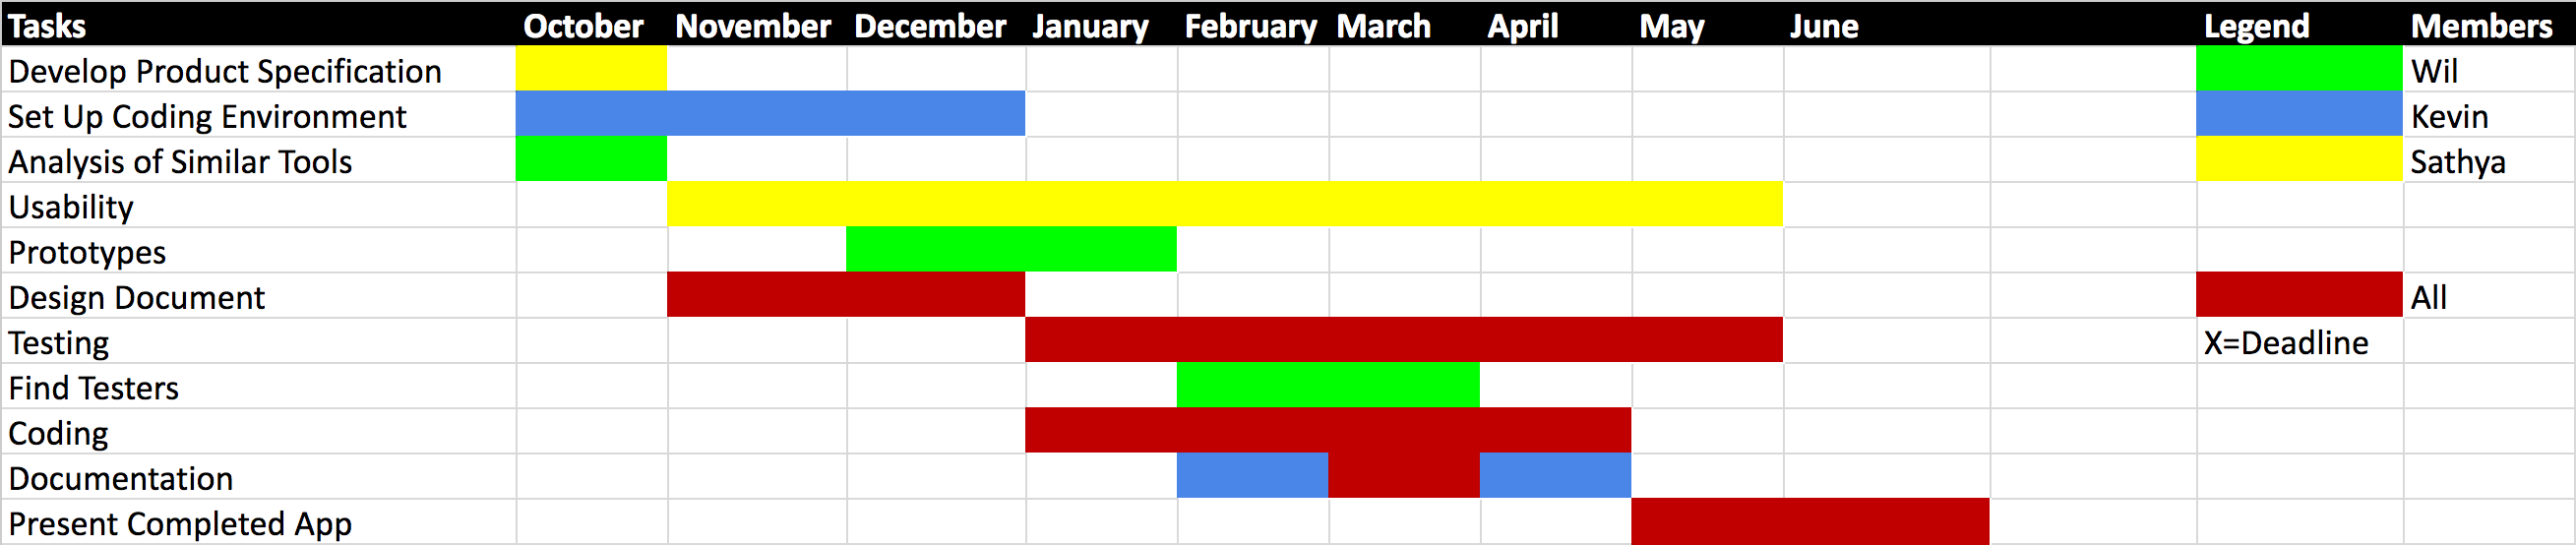
\includegraphics[scale=.5]{ganttChart.png}  
    \caption{\label{fig:Development Timeline}Development Timeline.} 
\end{sidewaysfigure}

\backmatter
\end{document}
